\documentclass{article}
\usepackage[utf8]{inputenc}
\usepackage[total={6.5in,9in}]{geometry}
\usepackage{xcolor,graphicx}

\newcommand{\FJH}[1]{{\color{blue}Fred: #1}}
\newcommand{\ny}[1]{{\color{brown}Yiou: #1}}
\newcommand{\yuhannote}[1]{{\color{purple}Yuhan: #1}}


\title{Proposal for the \\
15th International Conference on Monte Carlo Methods and Applications (MCM)\\
MCM 2025 in Chicago, IL USA}
%\author{jinliang98}
%\date{February 2022}

\begin{document}

\maketitle

\section{Summary of the proposal}
The \FJH{Write}

\section{Local organizers}
 The organizing team represents different thematic currents in the
community, both on theoretical, numerical and application aspects.
\begin{itemize}
    \item  Fred Hickernell, Applied Mathematics, Illinois Institute of Technology
    \item  Lulu Kang, Applied Mathematics, Illinois Institute of Technology
    \item  Yuhan Ding, Applied Mathematics, Illinois Institute of Technology
    \item  David Minh, Chemistry, Illinois Institute of Technology
    \item  Yiou Li, Mathematical Sciences, DePaul University
\end{itemize}

\section{Program Committee}
The program committee will be an international and multidisciplinary in nature.  It will be drawn from those who have had a history of contribution to the MCM series plus those whose expertise may add a valuable dimension to the conference.

\section{Proceedings}

\FJH{Need to discuss with committee}

\section{Conference Venue}

The conference will be held at Illinois Tech Hermann Hall. 
A conference dinner on the Chicago River or at Chinatown with a night architecture tour will be organized.

\section{Tentative Dates and Schedules}

July 28th to August 1st 2025
\yuhannote{Discuss with committee}

The dates will be finalized to avoid overlap with the 2025 SIAM Annual Meeting, the August 2 – 7, 2025, Joint Statistics Meeting, 
5 days conference with the following format for each day
\begin{itemize}
    \item  Morning: keynote speaker (1h), parallel mini-symposia (2h)
    \item  Afternoon: keynote speaker (1h), parallel mini-symposia (2h)
\end{itemize}
Poster sessions: at the lunch breaks
\begin{figure}[h]
    \centering
    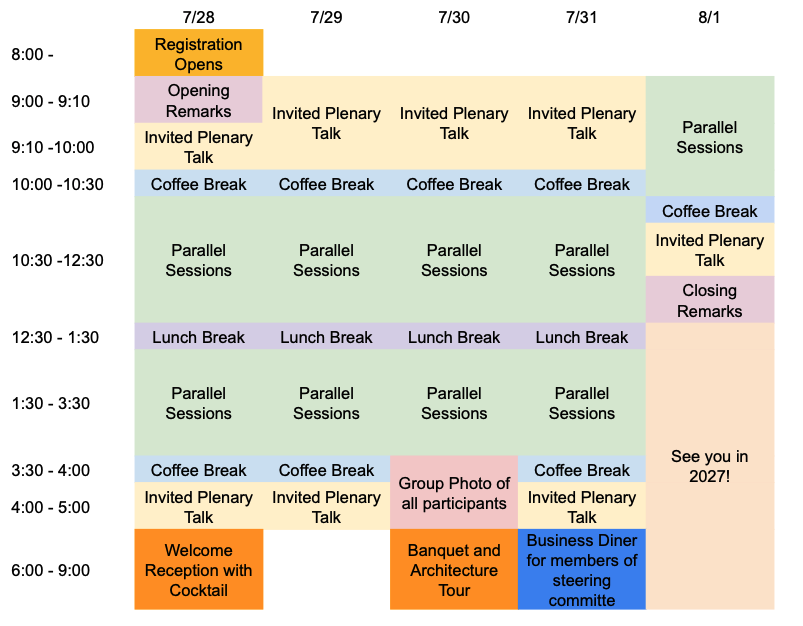
\includegraphics[width =.95\textwidth]{schedulev2.png}
    \caption{Tentative Schedule}
\end{figure}

\section{Topics}
The MCM Conference is a biennial meeting on Monte Carlo and quasi-Monte Carlo methods.
The conference will be open to usual active topics of MCM conferences, but we will
also make effort to include emerging topics coming from applications.  It focuses on recent research related to the following topics:
\begin{itemize}
\item Markov chain Monte Carlo
\item Hamiltonian Monte Carlo
\item Sequential Monte Carlo, particle filters
\item Non-equilibrium candidate Monte Carlo
\item Bridge sampling
\item Rare event simulation
\item Multi-level Monte Carlo
\item (Randomized) Quasi-Monte Carlo
\item Digital nets and lattice rules
\item Discrepancy theory
\item Complexity and tractability of multivariate problems
\item Variance reduction
\item Monte Carlo Simulation on High-Performance Architectures
\item Uncertainty quantification
\item Experimental design
\item Generative models from artificial intelligence
\item Variational inference
\item Probabilistic numerics
\item Monte Carlo methods for quantum computers
\item Stochastic gradient and other stochastic optimization methods
\item Statistical learning and Monte Carlo sampling
\item Reinforcement learning and control
\item Bayesian Inference
\item Computational statistical physics
\item Economic, Engineering, Industrial, and Scientific Applications
\end{itemize}

\ny{The logic is: (1) sample generation; (2) improving the performance; (3) applications in fields other than classical numerical integration. 

The major changes are: (1) particle methods $->$ particle filters; (2) non-equilibrium Monte Carlo $->$ non-equilibrium candidate Monte Carlo; (2) combine ``Bayesian inference" and ``variational methods" to ``variational Bayesian inference". 

My question is: It seems Hamiltonian Monte Carlo is a method of MCMC. Should we list it as a separate topic?}


\section{Budget}
The registration fees would be USD600/person including the conf. dinner, coffee/lunch breaks. Only expenses from keynote speakers will be covered. Expected number of participants is 150. For students, the registration fees would be USD250/person. Expected number of students is 50. The sponsorship will come from our collaborators: IMSI, CISC, and the Center for Stochastic Dynamics and Computation.

%Jeanette R. Massura, Director, Event Services, jmassura@iit.edu

%Ken Johnston, Interim Controller, 312.567.5850 johnston@iit.edu




\begin{figure}[h]
    \centering
    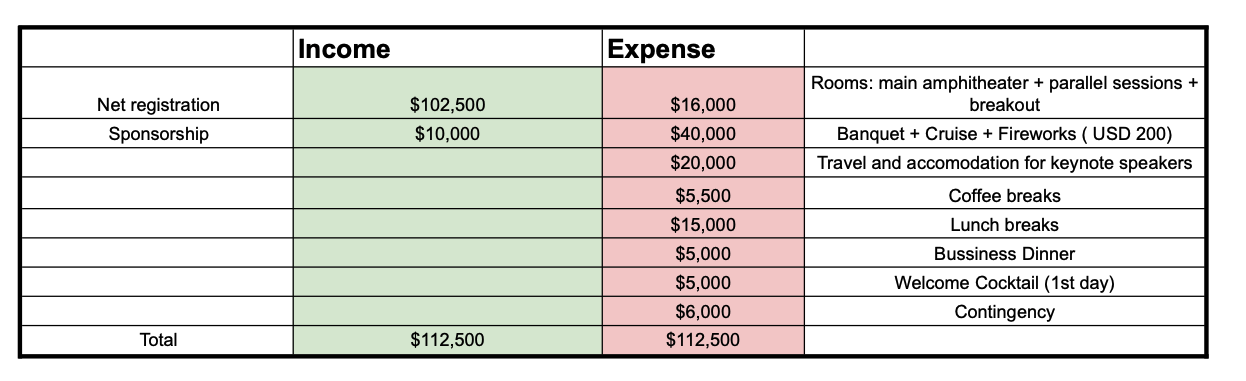
\includegraphics[width =.95\textwidth]{budgetv3.png}
\end{figure}


\section{History of conferences}
\begin{itemize}
\item Paris, France, July 2023
\item  Mannheim, Germany, August 2021
\item Sydney, Australia, July 2019
\item Montreal, Canada, July 2017
\item  Linz, Austria, July 2015
\item  Annecy-le-Vieux, France, July 2013
\item  Borovets, Bulgaria, August 2011
\item  Brussels, Belgium, September 2009
\item  Reading, UK, June 2007
\item  Tallahassee, USA, May 2005
\item  Berlin, Germany, September 2003
\item  Salzburg, Austria, September 2001
\item  Varna, Bulgaria, June 1999
\item  Brussels, Belgium, April 1997
\end{itemize}


\end{document}
